\section{Framework of a centralized and decentralized system}
When looking at the traditional pyramid, which is fully centralized, it seems difficult, if not impossible to translate this to a decentralized solution \todo[REf naar begin]{Ref naar begin}. And it should be possible to determine whether a centralized or decentralized solution, using a MAS or holonic system, should be implemented at a business process. A framework to compare a centralized versus a decentralised solution is discussed here. Essential in the difference between these two possible solution spaces is the location of the processing power for the calculations. Centralised solutions have a single control unit where the information flows to, while decentralized solutions do not have this structure.

A popular comparison, discussed by \citet{parunak1999industrial}, is that of the original Roman army structures. Decisions where made at the top and dripped down, while the information stream went up. This method has been deployed in most companies. Due to the fact that something can be computed on a single computer, and be optimized on this single program, an optimal decision can be found.

However, the increasing complexity of computer and information systems, combined with the increasing complexity of their applications, exceed the level of conventional centralized computing. This is due to the processing of huge amounts of data, or data that originate from different locations. To solve such difficulties, computers have to act more like agents where each agent can solve, or decide on part of the problem. This is where agent-based architectures are an ideal fit to such a decentralized organizational structure.

To push the decision making to the lowest level, excessive layers of management can be obsolete. This allows for, sometimes, easier to understand and developing of problems, especially if the problem being solved is itself distributed.

By using principles of decomposition which is a classical optimization (reformulation) method \citep{sharif2012yard} presents a comparative study of two contrasting approaches for modelling the yard crane scheduling problem: centralized and decentralized. It seeks to assess their relative performances and factors that affect their performances. They conclude that a centralized approach outperforms the decentralized approach by 16.5 \% on average, due to having complete and accurate information about future truck arrivals. However, since the decentralized under performs the centralized, the decentralized approach can dynamically adapt to real-time dynamic changes, making it better suited for real-life operations. 

To optimize these different types of resources allocation problems, there are different kinds of allocation problems, for which different solutions are feasible. The purpose here is to find what characteristics are optimal to use a centralized vs a decentralized solution.

%\begin{figure}
%\centering
%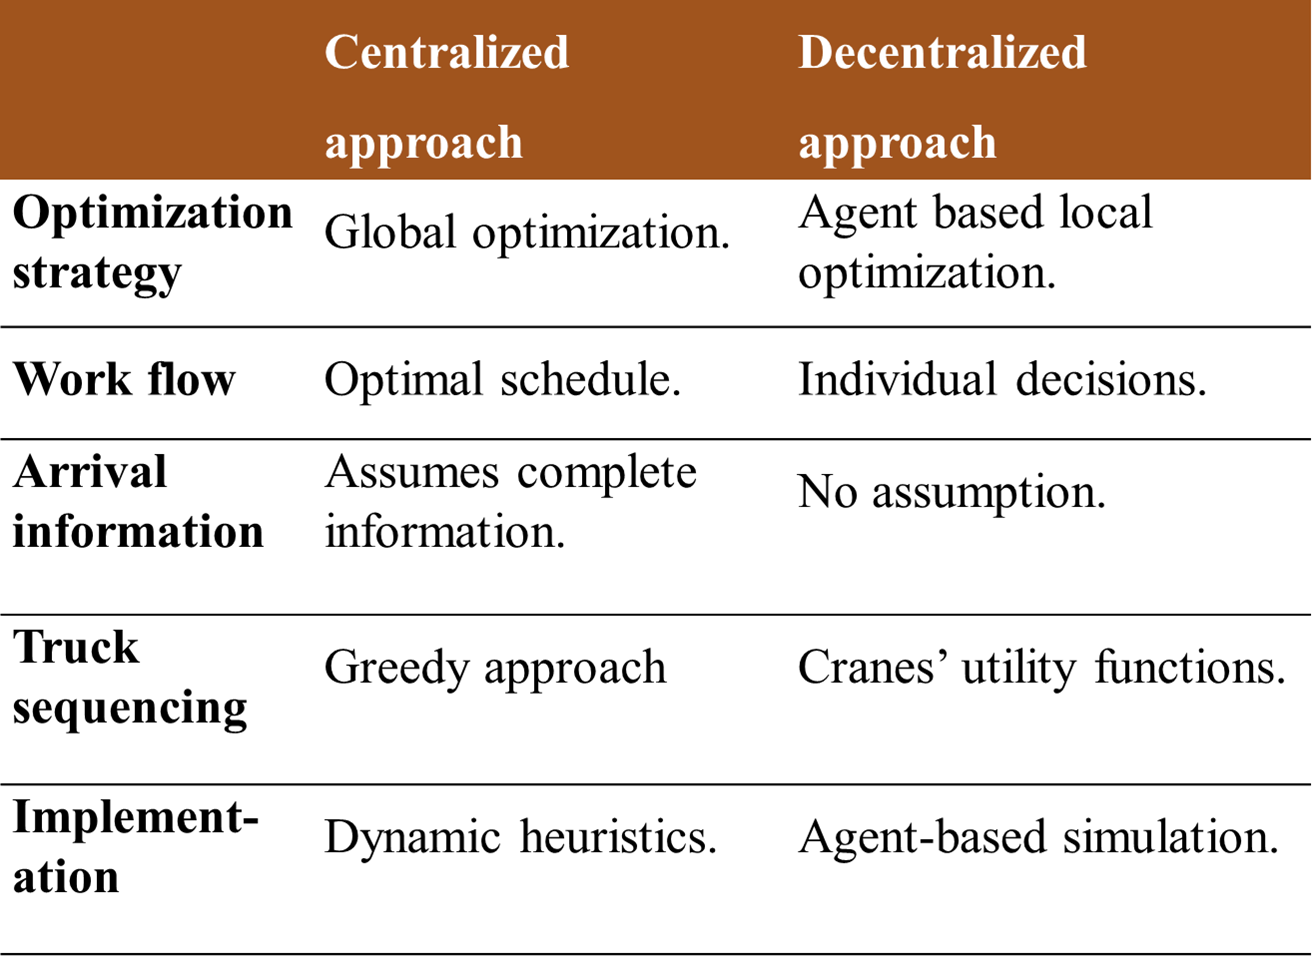
\includegraphics[width=0.7\linewidth]{img/yard_compare_ca_da}
%\caption{}
%\label{fig:yardcomparecada}
%\end{figure}



% The increasing complexity of computer and information systems goes together with an increasing complexity of their applications. These often exceed the level of conventional, centralized computing because they require, for instance, the processing of huge amounts of data, or of data that arises at geographically distinct locations. To cope with such applications, computers have to act more as \individuals" or agents, rather than just \parts."

%centralized solutions are generally more efficient: anything that can be computed in a distributed system can be moved to a single computer and optimized to be at least as efficient. However, distributed computations are sometimes easier to understand and easier to develop, especially when the problem being solved is itself distributed. Distribution can lead to computational algorithms that might not have been discovered with a centralized approach. There are also times when a centralized approach is impossible, because the systems and data belong to independent organizations that want to keep their information private and secure for competitive reasons.


\subsection{Size and modularity}
A critical aspect of the possibility to determine whether a centralized or decentralised solutions is preferred is the search space size of the problem. The size of the problem is seen as the number of resources or task that have to be allocated.  If a clear structure is conceivable and a clear population is in place a centralized solution is infeasible. This is due to the global overview. However, the high sensitivity to size and complexity makes a centralized solution impracticable.


%Since a centralized solutions are highly sensitive to the size and complexity and require performing the computation in advance, they lack the dynamically needed in real-life situations. The decentralized Approach dont require computation time required in advance and can use disaggregated, handle large and complex problems

%\subsection{Modularity}
In a decentralized structure, individual models are decoupled from one another, errors in one module impact only those modules that interact with it, leaving the rest of the system unaffected. This can be seen in \Cref{fig:modularitydecentral-changeability}. It shows however the importance of having a clear modular problem. 

\todo[ge copy past!]{Ge copy paste!}
Distributed Problem Solving
Imagine a multiagent system inhabited by several agents with different
problem solving capabilities. A particular complex problem may not be
solvable by any single agent, but possibly by several agents together.
• Problem decomposition: Decompose the original problem into
smaller subproblems, that can each be handled by a single agent.
• Solving each subproblem: Each agent solves the problems
assigned to them. Agents may share information during this stage.
• Solution synthesis: Integrate the solutions to the subproblems to
arrive at a solution of the overall problem.
In this strand of work people generally assume that agents are
cooperative and benevolent . . . Negotiation as a Metaphor for Distributed Problem
Solving

Centralised vs. Distributed Approaches
So far we have concentrated on auctions as mechanisms for solving
resource allocation problems. But what if we cannot find someone who
could act as the auctioneer?
• The associated tasks may be too hard computationally for the
agent supposed to assume the role of auctioneer.
• There may be no agent that enjoys the trust of the others.
• The system infrastructure may be truly distributed and it may
simply be unnatural to model the problem in a centralised manner.
• The goods may be owned by different agents to begin with
(that is, we may have to take an initial allocation into account).
• Agents and goods may enter or leave the system dynamically.
Auctions are centralised mechanisms. All of the above are good
reasons to consider distributed negotiation schemes as well .

%As Figure 9.1 suggests, in a system with a single thread of control, changes to a single module can cause later modules, those it invokes, to malfunction. Decentralization decouples the individual modules from one another, so that errors in one module impact only those modules that interact with it, leaving the rest of the system unaffected. (The original version of this gure was created by Seiichi Yaskawa of Yaskawa Electric Corporation, Tokyo, Japan, and is used with his kind permission.)

\begin{figure}[h]
\centering
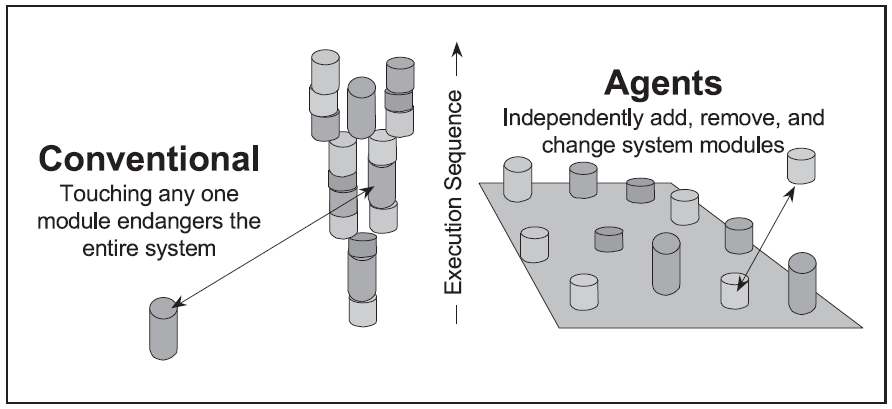
\includegraphics[width=0.7\linewidth]{img/modularity+decentral-changeability}
\caption{Comparison of a conventional control thread and an agent-based control, from \citep{parunak1999industrial}.}
\label{fig:modularitydecentral-changeability}
\end{figure}



\subsection{Dynamicity (Time Scale/Changeability)}
In a centralized solution, the continuous monitoring of the state of the environment and typically the lack of complex decisions, a quick reaction to changes is possible. A high dynamical is the result. 

Unfortunately, it is difficult to achieve real-time scheduling in traditional manufacturing systems because the scheduling algorithms used are executed on a single, centralized computer that becomes computational incredibly difficult \citep{duffie1994real}.
\subsection{Solution Quality}
Since agent-based approaches are distributed, they do not have a global view of the entire state of a system. A lot can reached through communication and negotiation, but for a truly optimal solution, an entire view is necessary For example,  \citep{palmer2003decentralized} shows that this algorithm is not intended to find the optimal solution; it finds a good solution with less computation. 

In the centralized approach the assumption of a complete information on supply and demand is made. This requires rescheduling to adapt with changes. In the decentralized approach, no assumptions on the complete information is necessary. 

New advances however, like this research have tried to find an optimal centralized solution. 
%Adaptability
%Centralized Approach
%Assumes complete information on supply and demand
%Requires rescheduling to adapt with changes
%Decentralized Approach
%No assumptions on the arrival-time of trucks
%Monitor changes continuously, adapt rapidly


\subsection{Complexity}
Since an agent can execute actions only on its own surrounding, it is dependent on its local parameters. However, the agent can use information sent by its neighbours to adapt \citep{pujolle2006autonomic}. This interaction between the elements makes the complexity of a solution many times higher and more difficult than a centralized solution.

\subsection{Framework overview}
\begin{tabular}{p{2cm}|p{2.5cm}|p{2.5cm}|p{2.5cm}}
	& Centralised Solution & Decentralised Solution & Building Blocks\\
	\hline \hline
	Size / Modularity & Small; No sub-problems & Large; Ill-Structured; Easily dividable; Independent Modules & Population; Holonic; number of resources: (decision variables, parameters \& constraints)\\
	\hline
	Time scale / Changeability & Days - Weeks; Not subject to a lot of change & Real-time - Hour; Changeability  & Adaptive Capability ; Degree of Re- and Pro-activeness\\
	\hline
	Solution quality & Perfect & (sub-)Optimal & Object and Solution Space\\
	\hline
	Complexity & Simple & Complex & Interaction between the set of elements; Communication
\end{tabular}

%To achieve the autonomic-oriented architecture, we propose to select the appropriate control mechanisms among: 
%- adaptive: the agent adapts its actions according to the incoming events and to its vision of the current system state. The approach we propose is adaptive as the agent adapts the current control mechanisms and the actions undertaken when a certain event occurs. The actions the control mechanism executes may become no longer valid and must therefore be replaced by other actions. These new actions are indeed more suitable to the current observed state;
%- distribution: each agent is responsible for a local control. There is no centralization of the information collected by the different agents, and the decisions the agent performs are in no way based on global parameters. This feature is very important as this avoids having bottlenecks around a central control entity;
%- local: the agent executes actions on the elements of the node it belongs to. These actions depend on local parameters. However, the agent can use information sent by its neighbours to adapt the activated control mechanisms;
%- scalable: the proposed approach is scalable because it is based on a multi-agent system which scales well with the growing size of the controlled network. In order to adaptively control a new node, one has to integrate an agent (or a group of agents) in this node to perform the control. 
